Damit ihr nicht ganz verloren im gro\ss en Uni-Wirrwarr umher irrt und
  nicht immer das Gefühl haben müsst, etwas sehr Wichtiges geht
  voll an euch vorbei, findet ihr hier eine Übersicht über die wichtigsten Begriffe:

\begin{description}

\item [Übungen:] Zu den Mathe- und Informatikvorlesungen werden neben den Vorlesungen noch Übungsblätter angeboten, welche euch helfen, den gelernten Stoff zu verinnerlichen. Meist könnt ihr über die Übungsblätter, die ihr wöchentlich oder zweiwöchentlich abgeben könnt, einen Bonus für eure Klausurnote erarbeiten. In machen Vorlesungen kann aber auch eine Mindestpunktzahl in den Übungen Voraussetzung für die Klausur sein.

Da die dazu zu lösenden Aufgaben manchmal recht heftig und zeitaufwändig ausfallen, empfiehlt es sich:

\begin{itemize}

\item \textbf{sofort voll einzusteigen}, denn die Aufgaben werden von Mal
  zu Mal schwerer.

\item sich eine \textbf{Arbeitsgruppe} zu suchen, denn alleine ist man
  als "`Normalbegabter"' fast verloren. Meistens darf eine
  Arbeitsgruppe (2-3 Studis) sogar eine gemeinsame Lösung abgeben!

\item auch dann Übungen zu machen, wenn es keine Pflichtaufgaben sind --
  die Klausur kommt bestimmt.

\end {itemize}

\begin{center}
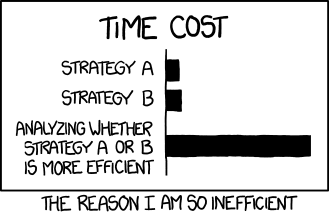
\includegraphics[width=0.5\hsize]{info/xkcd/efficiency.png}
\end{center}


(Don't panic -- Die Matheübungszettel sind zu Anfang zwar der gro\ss e
  Schocker, die Prüfungen laufen aber in gemä\ss igterem Rahmen ab.)

\item [Vorlesungen:] In den Vorlesungen wird euch der nötige Stoff vermittelt. Es empfiehlt sich bei jeder Vorlesung sich Notizen zu machen und die Vorlesung nachzuarbeiten, da die Notizen oft chaotisch und unübersichtlich sind. Welche Vorlesungen angeboten werden findet ihr im Vorlesungsverzeichnis.	%TODO insert \link{}{}?

\item [Vorlesungsverzeichnis:] Eine Übersicht über alle Veranstaltungen der Universität findet ihr in ALMA\footnote{\link{https://alma.uni-tuebingen.de}{ALMA}}. Dort findet ihr auch später eine Übersicht über eure Noten und könnt euch Studienbescheinigungen runterladen. Außerdem finden hier die Anmeldungen zu den Klausuren statt.	%TODO insert \link{}{}?

\item [ECTS, Credits, LP:] ECTS-Punkte (European Credit Transfer System, auch \textit{Credits} oder \textit{Leistungspunkte, LP}) sind seit der europaweiten Standardisierung von Bachelor- und Masterstudium (Bologna-Prozess\footnote{\url{https://de.wikipedia.org/wiki/Bologna-Prozess}}) die Währung, in der Leistung gemessen wird. 1 ECTS-Punkt entspricht ca. 30 Stunden Arbeit. Gibt eine Vorlesung 3 ECTS-Punkte, so müsst ihr in dem Semester ca. 90 Stunden für diese Vorlesung investieren. Habt ihr in den 15 Semesterwochen je zwei Stunden Vorlesung (also $15\cdot 2=30$ Stunden) durch Präsenzzeit investiert, so solltet ihr noch ca. 60 Stunden im Semester selbstständig für die Vorlesung investieren, um auf die vorgesehenen 90 Stunden zu kommen (vorbereiten, nachbereiten, zusammenfassen, auf die Klausur lernen).\\	%TODO insert \link{}{}?
Die Noten der jeweiligen Veranstaltungen werden mit deren ECTS-Punkten gewichtet.
 
\item [Eduroam:] Eduroam ist ein europaweiter Verbund von Bildungseinrichtungen, welcher es ermöglicht, an allen teilnehmenden Bildungseinrichtungen mit demselben Login ins Internet zu gehen.
Eine Anleitung, wie man Eduroam richtig einrichtet findet ihr im Infrastruktur-Kapitel.

\item [ZDV:] Das Zentrum für Datenverabeitung (ZDV) ist das Rechenzentrum der Universität und betreut die zahlreichen Rechner und Server, welche auch von Studierenden genutzt werden können. Vom ZDV solltet ihr nach eurer Immatrikulation auch ein Schreiben mit eurem ZDV Benutzernamen und einem Passwort bekommen haben. Diese ermöglichen euch die Nutzung der Uni-Infrastruktur.

\item [CIP Pool:] CIP Pools sind von der Universität betriebene Räume in denen Rechner des ZDVs stehen, die man als Studierender mit seiner ZDV Kennung nutzen kann.

\item[BAföG:] Das Bundesausbildungsförderungsgesetz unterstützt Studierende und Auszubildende aus einkommensschwachen Elternhäusern. Ob und wie ihr BAföG bekommt könnt ihr hier nachschauen: \url{http://www.bafoeg-rechner.de/}	%TODO insert \link{}{}?

\item[Mensa:] Die Mensen sind der Ort in dem man sich zum (un-)regelmäßigen Mittagessen trifft. Jede Mensa hat einen Speiseplan, welchen man auf der Seite des Studierendenwerks einsehen kann\footnote{\url{http://www.my-stuwe.de/mensa/}}.	%TODO insert \link{}{}?

\vfill

\end{description}
\pagebreak
